\chapter{Your Contribution}
\label{ch:ownwork}

%%%%%%%%%%%%%%%%%%%%%%%%%%%%%%%%%%%%%%%%%%%%%%%%%%%%%%%%%%%%%%%%%%%%%%%%
\section{Approach}
\label{sec:approach}

Describe your approach, design, or methodology. Explain the decisions you made and justify them. Figures and tables should be used to support your explanation.

\subsection{Design}
\label{sec:design}

Describe each of these:
\begin{itemize}
  \item Hardware: Gaia HPC Cluster 
  \item Solver: Synxflow
  \item Soft Sensor: Alumet (Isolates energy consumption by process-level GPU/CPU utilization percentages.)
\end{itemize} 

\begin{figure}[ht]
  \centering
  % Replace with your own figure in the Images/ folder:
  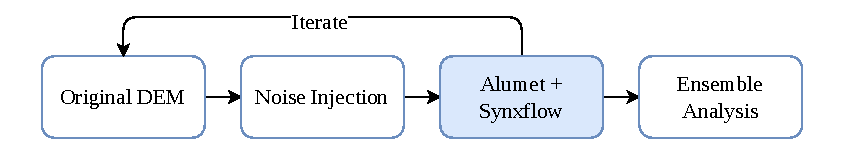
\includegraphics[width=1\textwidth]{images/Workflow.pdf}
  \caption{Computational Pipeline Flowchart}
  \label{fig:design}
\end{figure}

\subsection{Mathematical Formulation}
\label{sec:math}

\begin{itemize}
  \item The artificial topographical noise, which simulates uncertainty, is modeled using a Gaussian probability density function ~\eqref{eq:pdf}.
  \item The mean error is set to zero ($\mu = 0$), assuming that the surveying equipment has no systematic directional bias.
  \item $\sigma$ is the variable controlling the intensity of the simulated sensor noise. The specific discrete levels tested in ensembles are: $\sigma \in \{0.05, 0.1, 0.2, 0.5, 1.0\}$ meters.
  \item The generated noise matrix, defined by $\mathcal{N}(0, \sigma^2)$, is added cell-by-cell to the original DEM elevation matrix to generate the equiprobable realizations.
\end{itemize}

\begin{equation}
f(x) = \frac{1}{\sigma\sqrt{2\pi}} \exp\left(-\frac{(x - \mu)^2}{2\sigma^2}\right)
\label{eq:pdf}
\end{equation}

\subsection{Implementation}
\label{sec:implementation}

\begin{itemize}
  \item All parameters such as boundary conditions, landcover friction values, and temporal settings for the solver are exported from a YAML configuration file to ensure easier experiment reproducibility. 
  \item Synxflow solver is executed as a subprocess wrapped by Alumet. The unique process ID (PID) is identified and extracted from the terminal log file, enabling the isolation of the energy.
  \item Since the energy counters on the CPU and GPU hardware are asynchronous, the post-processing algorithm uses interpolation to match the energy telemetry to a unified timeline.
  \item The Quantity of Interest (QoI) water depth at a specific location is sampled for each iteration. The energy consumption for each iteration is calculated based on the interpolated energy telemetry.
  \item The resulting variance and uncertainty are represented visually using Kernel Density Estimation (KDE) using scipy.stats and matplotlib.
\end{itemize}